\documentclass{beamer}
\mode<presentation> {
\usetheme{Antibes}
\usecolortheme{crane}
\setbeamertemplate{footline}[page number]
}
 
\usepackage{graphicx}
\usepackage{booktabs} 
\usepackage{enumerate}
\usepackage{physics}
\setbeamerfont{caption}{size=\footnotesize}

 
\title[Matrix Project]{Matrices in Coordinate Geometry}
 
\author{Karthik Pagadala (EE17BTECH11049)\\Dhruv Gupta (EP17BTECH11006)}
\institute[IITH] 
{
Indian Institute Of Technology Hyderabad \\
\medskip
EE1390 Matrix Project
}

\date{\today} 
 
\begin{document}
 
\begin{frame}
\titlepage
\end{frame}
 
\begin{frame}
\frametitle{Overview}
\tableofcontents 
\end{frame}

%------------------------------------------------
\section{The Original Problem}
%------------------------------------------------
 
\begin{frame}
\frametitle{The Original Problem}
JEE (Advanced)2018 - Paper 1 - Q.3
\noindent\makebox[\linewidth]{\rule{\paperwidth}{0.4pt}}
Let $P_{1}: 2x + y - z = 3$ and $P_{2}: x + 2y + z = 2$ be two planes. Then, which of the following statement(s) is(are) TRUE?
\begin{enumerate}[(A)]
    \item The line of intersection of $P_{1}$ and $P_{2}$ has direction ratios $1,2,-1$
    \item The line
    \[
    \frac{3x-4}{9} = \frac{1-3y}{9}=\frac{z}{3}
    \]
    is perpendicular to the line of intersection of $P_{1}$ and $P_{2}$
    \item The acute angle between $P_{1}$ and $P_{2}$ is 60$^\circ$
    \item If $P_{3}$ is the plane passing through the point $(4,2,-2)$ and perpendicular to the line of intersection of $P_{1}$ and $P_{2}$, then the distance of the point $(2,1,1)$ from the plane $P_{3}$ is $\tfrac{2}{\sqrt{3}}$
\end{enumerate}
\end{frame}
 
%------------------------------------------------
\section{Matrix Transformation}
\begin{frame}
\frametitle{Matrix Transformation}
We can transform the problem into matrices in the following way
\begin{itemize}
\item<1-> The plane can be written in the form 
    \[
    \vec{n}\cdot\vec{x}=d
    \]
\item<2-> The direction vector of a line in the form: 
    \[
    \frac{x-x_{1}}{a}=\frac{y-y_{1}}{b}=\frac{z-z_{1}}{c}
    \] is $\vec{L}(a,b,c)$
\end{itemize}
\end{frame} 
%--------------------------------------------------
\section{Solution}
\subsection{Line Of Intersection of Planes}
\begin{frame}
\frametitle{Solution}

(A) To find the direction ratios of the line of intersection of $P_{1},P_{2}$
\begin{itemize}
\item<1-> The two planes have normal vectors $n_{1},n_{2}$
\item<2-> The cross product, $n_{1}\times n_{2}$ will give us the direction vector of the line of intersection
\item <3->
\[  n_{1}=
    \begin{bmatrix}
    $2$\\$1$\\$-1$
    \end{bmatrix}
    ,n_{2}=
    \begin{bmatrix}
    $1$\\$2$\\$1$
    \end{bmatrix}
\]
\item <4->
\[
    n_{1}\times n_{2}=
    \begin{bmatrix}
    n_{12}n_{23}-n_{13}n_{22} & n_{13}n_{21}-n_{11}n_{23} & n_{11}n_{22}-n_{12}n_{21}
    \end{bmatrix}^{T}
\]
\item <5->
\[
    n_{1}\times n_{2}=
    \begin{bmatrix}
    3 & -3 & 3
    \end{bmatrix}^{T}
\]
\item<6-> The resultant ratio can be compared to the given direction ratios
\end{itemize}
\end{frame}

%------------------------------------------------
\begin{frame}
\frametitle{Solution}

(B) To test if line of intersection of $P_{1},P_{2}$ is perpendicular to given line 
\begin{itemize}
\item<1-> The two planes have normal vectors $n_{1},n_{2}$ and let line of intersection have direction vector $L_{1}(3,-3,3)$
\item<2-> The direction ratios of the line $L_{2}$
\[
    \frac{3x-4}{9} = \frac{1-3y}{9}=\frac{z}{3}
\] are $d: (2,-2,1)$
\item<3-> If $L_{1}$ is $\perp$ to $L_{2}$, it is implied to be co-planar with $P_{1},P_{2}$.
\item<4-> Use Scalar Dot Product to check the above.
    \[
        d\cdot(n_{1}\times n_{2})=
        \begin{bmatrix}
        2 & -2 & 1
        \end{bmatrix}
        \cdot
        \begin{bmatrix}
        1\\-1\\ 1
        \end{bmatrix}
        = 5 \neq 0
        
    \]
\end{itemize}
\end{frame}
 
%------------------------------------------------
 \subsection{Angle Between Planes}
\begin{frame}
\frametitle{Solution}

(C) Finding the angle between planes
\begin{itemize}
\item<1-> The angles between the planes is the same as the angle between normal vectors $\vec{n_{1}},\vec{n_{2}}$
\item<2-> The angle is given by
    \[
    \vec{n_{1}}\cdot\vec{n_{2}} =\norm{\vec{n_{1}}} \norm{\vec{n_{2}}} \cos \theta
    \]
    \[
    \theta = \arccos{\frac{\begin{bmatrix}2 & 1 & -1\end{bmatrix}\cdot \begin{bmatrix}1\\2\\1\end{bmatrix}}{\sqrt{6}\cdot\sqrt{6}}} = 60^\circ
    \]
    
    
\end{itemize}
\end{frame}

%---------------------------------------------
 \subsection{Distance Between Point \& Plane}
 \begin{frame}

\frametitle{Solution}

(D) Distance Between Point and Plane
\begin{itemize}
\item<1-> The component of the vector joining $A(4,2,-2)$ and $P(2,1,1)$ along the normal $n_{3}$ is the distance between the point and plane.
\item <2->\[
    dist = \abs{\frac{n^{T}\cdot (A-P)}{\norm{n}}}
\]
\item<3-> \[
    dist = \abs{\frac{\begin{bmatrix}3 & -3 & 3\end{bmatrix}\cdot(
    \begin{bmatrix}4\\2\\-2\end{bmatrix}-
    \begin{bmatrix}2\\1\\1\end{bmatrix})
    }{\sqrt{27}}} = \frac{2}{\sqrt{3}}
\]
\end{itemize}
\end{frame}
 

\section{Figures}

\begin{frame}
\frametitle{Figures}
\begin{figure}[H]
    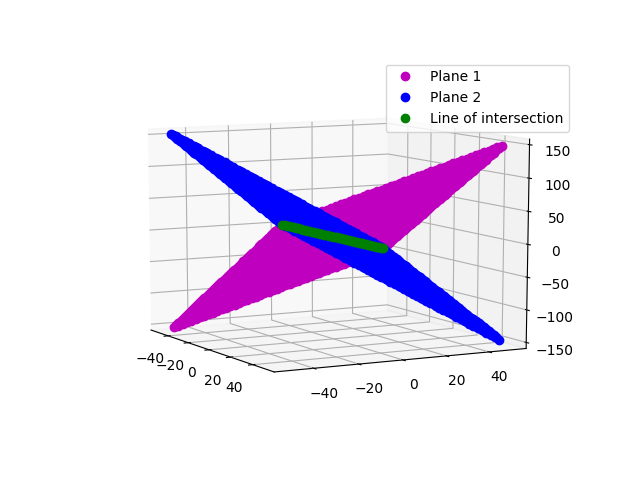
\includegraphics[width=0.7\textwidth,keepaspectratio, trim =2cm 2cm 1cm 1.5cm, clip]{/home/dhruvg/Desktop/EE1390/figs/A1.png}
    \caption{A - Planes \& Line Of Intersection}
    \label{A}
\end{figure}
\end{frame}
%------------------------------------------------
 
\begin{frame}
\frametitle{Figures}
\begin{figure}[H]
    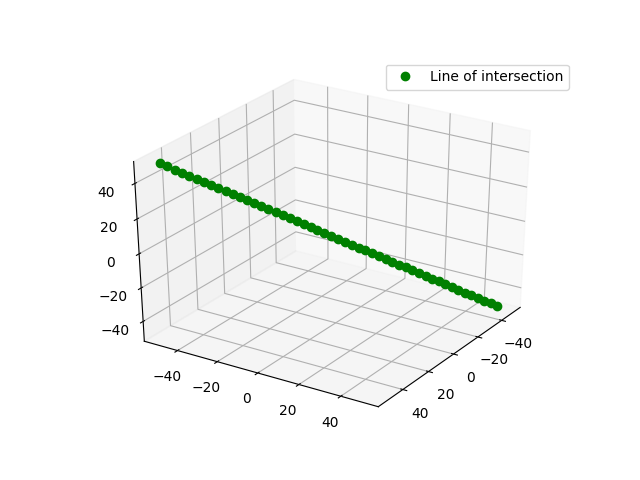
\includegraphics[width=0.7\textwidth,keepaspectratio, trim =1cm 1cm 1cm 1.5cm, clip]{/home/dhruvg/Desktop/EE1390/figs/A2.png}
    \caption{A - Line Of Intersection}
    \label{A}
\end{figure}
\end{frame}
 
%----------------------------------------------------------------------------------------

\begin{frame}
\frametitle{Figures}
\begin{figure}[H]
    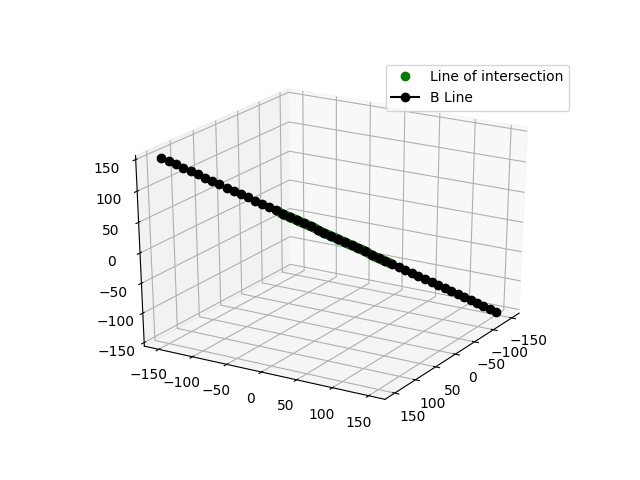
\includegraphics[width=0.7\textwidth,keepaspectratio, trim =1cm 1cm 1cm 1.5cm, clip]{/home/dhruvg/Desktop/EE1390/figs/B1.png}
    \caption{B- Line In Question}
    \label{B}
\end{figure}
\end{frame}

%----------------------------------------------------------------------------------------

\begin{frame}
\frametitle{Figures}
\begin{figure}[H]
    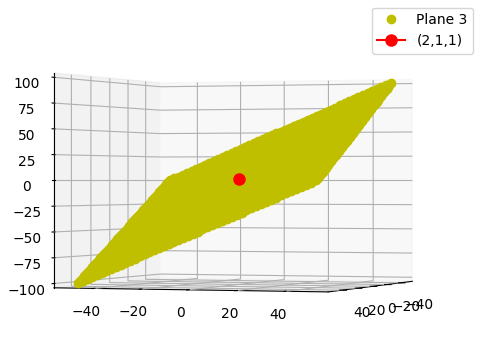
\includegraphics[width=0.7\textwidth]{/home/dhruvg/Desktop/EE1390/figs/D1.png}
    \caption{D- Point and Plane}
    \label{D}
\end{figure}
\end{frame}


\begin{frame}
\frametitle{Figures}
\begin{figure}[H]
    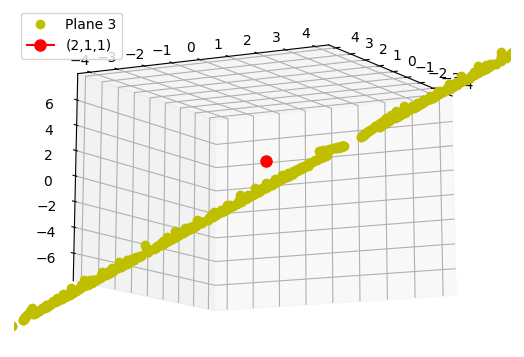
\includegraphics[width=0.7\textwidth]{/home/dhruvg/Desktop/EE1390/figs/D2.png}
    \caption{D- Point and Plane}
    \label{D}
\end{figure}
\end{frame}


\begin{frame}
\frametitle{Figures}
\begin{figure}[H]
    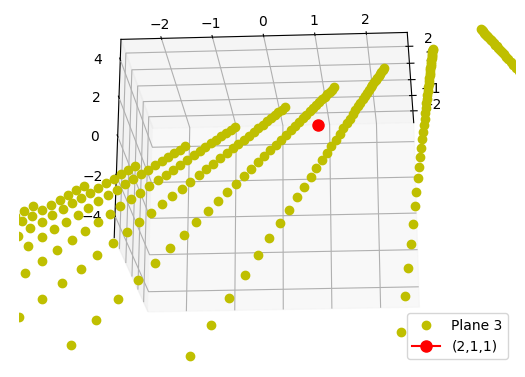
\includegraphics[width=0.7\textwidth]{/home/dhruvg/Desktop/EE1390/figs/D3.png}
    \caption{D- Point and Plane}
    \label{D}
\end{figure}
\end{frame}
 \begin{frame}
\Huge{\centerline{The End}}
\end{frame}
\end{document}
